\documentclass{article}

% Language setting
% Replace `english' with e.g. `spanish' to change the document language
\usepackage[english]{babel}

% Set page size and margins
% Replace `letterpaper' with `a4paper' for UK/EU standard size
\usepackage[letterpaper,top=2cm,bottom=2cm,left=3cm,right=3cm,marginparwidth=1.75cm]{geometry}

% Useful packages
\usepackage{amsmath}
\usepackage{graphicx}
\usepackage[colorlinks=true, allcolors=blue]{hyperref}

% My packages
\usepackage{listings}
% This file is part of https://github.com/Maumagnaguagno/Planning_LaTeX
\lstdefinelanguage{PDDL}
{
  sensitive=false,    % not case-sensitive
  morecomment=[l]{;}, % line comment
  alsoletter={:,-},   % consider extra characters
  morekeywords={
    define,domain,problem,not,and,or,when,forall,exists,either,
    :domain,:requirements,:types,:objects,:constants,
    :predicates,:action,:parameters,:precondition,:effect,
    :fluents,:primary-effect,:side-effect,:init,:goal,
    :strips,:adl,:equality,:typing,:conditional-effects,
    :negative-preconditions,:disjunctive-preconditions,
    :existential-preconditions,:universal-preconditions,:quantified-preconditions,
    :functions,assign,increase,decrease,scale-up,scale-down,
    :metric,minimize,maximize,
    :durative-actions,:duration-inequalities,:continuous-effects,
    :durative-action,:duration,:condition
  }
}
\lstset{language=PDDL}

\title{Solving Tower of Hanoi in PDDL}
\author{Mihnea Tîrcă}

\begin{document}
\maketitle

\tableofcontents
\pagebreak

\section{Introduction}

In this paper we will be solving the \emph{Tower of Hanoi} problem using \emph{Planning Domain Definition Language}. We will take a look at the game's rules (domain), as well as at our goal (problem). We will then transpose this problem into PDDL code. We will initially write the code for three disks (the original problem), and then we will try to generalize the problem by taking the number of disks as user input.

\section{The game}
The \emph{Tower of Hanoi} is a mathematical game or puzzle consisting of three rods and a number of disks of various diameters, which can slide onto any rod. The puzzle begins with the disks stacked on one rod in order of decreasing size, the smallest at the top, thus approximating a conical shape. The objective of the puzzle is to move the entire stack to the last rod, obeying the following rules:

\begin{enumerate}
    \item Only one disk may be moved at a time.
    \item Each move consists of taking the upper disk from one of the stacks and placing it on top of another stack or on an empty rod
    \item No disk may be placed on top of a disk that is smaller than it
\end{enumerate}

\begin{figure}[h!]
    \centering
    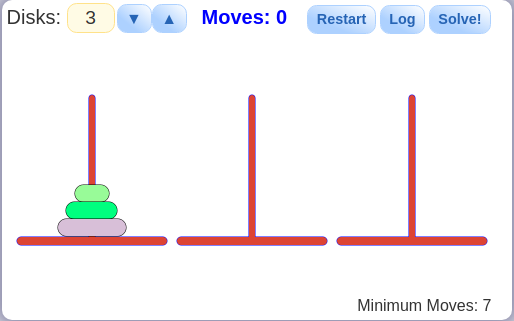
\includegraphics[scale=0.5]{"images/Initial_Position.png"}
    \caption{Tower of Hanoi starting position}
    \label{fig:init}
\end{figure}

\noindent
With 3 disks, the puzzle can be solved in 7 moves. The minimal number of moves required to solve a \emph{Tower of Hanoi} puzzle is \[2^n-1\], where \emph{n} is the number of disks. We will not be taking a look at the math, rather solving the problem using PDDL.\footnote{To get a better understanding of the game, try playing it \href{https://www.mathsisfun.com/games/towerofhanoi.html}{here}}

\section{Coding the three disks problem in PDDL}

\subsection{The domain}

To solve the problem using PDDL, we will first have to write the domain. We can think of the actions that we can take and then write the needed predicates accordingly. In theory, the only action that we can make is to move a disk. To move said disk to another tower, we would need to check if the disk is free (doesn't have another disk on top of it). So, we would need the predicate \emph{(on-top ?d ?t)}, which checks if disk \emph{d} is on top of tower \emph{t}. We would obviously need the predicate \emph{(smaller ?d1 ?d2)}, which checks if disk \emph{d1} is smaller than disk \emph{d2}, used when trying to move a disk on top of another. The predicates that I've found are needed are the following:

\begin{lstlisting}
(:predicates 
    (on-tower ?d ?t) ; disk d is on tower t (base of the tower)
    (on-disk ?d1 ?d2) ; disk d1 is on disk d2
    (disk ?d) ; d is a disk
    (tower ?t) ; t is a tower
    (empty ?t) ; tower t is empty
    (smaller ?d1 ?d2) ; disk d1 is smaller than disk d2
    (on-top ?d ?t) ; disk d is on top of tower t (free to move)
)
\end{lstlisting}

\noindent
For the the action of moving a disk, we need to state that once we've moved disk A that used to sit on disk B, disk B is now free. But what if we move disk A that does not sit on a disk? We would need to write a separate action for this scenario. Thus, the scenarios are:

\begin{enumerate}
    \item Moving a disk on top of a disk to a disk
    \item Moving a disk on top of a disk to an empty tower
    \item Moving a disk on an empty tower to a disk
    \item Moving a disk on an empty tower to an empty tower
\end{enumerate}

\noindent
To code these actions, we need to check multiple preconditions:

\begin{enumerate}
    \item The disk to move must always be free to move (on top of its tower).
    \item If we move the disk to an empty tower, we must check that is is in fact empty.
    \item If we move a disk \emph{A} that sits on top of another disk \emph{B}, disk B will be free after the move. Thus, we need to pass disk B as parameter and check in the preconditions if disk A sits on top of disk B. The effect will be that disk B is now free.
    \item If we move a disk to another disk, we need to check that the disk to be moved is smaller.
    \item If we move a disk from an empty tower, we need to check that it is at the base of its tower.
\end{enumerate}

\noindent
As for the effects, they are self-explanatory, given the preconditions.

\subsubsection{Moving a disk on top of a disk to an empty tower}

\begin{lstlisting}
; move disk from disk to tower
; ?d is the disk to move
; ?df is the disk under disk ?d
; ?t1 is the tower ?d is on
; ?t2 is the tower to move ?d to
(:action move-d-to-t
    :parameters (?d ?df ?t1 ?t2)
    :precondition (and 
        (disk ?d)
        (disk ?df)
        (tower ?t1)
        (tower ?t2)
        (empty ?t2)
        (on-disk ?d ?df)
        (on-top ?d ?t1)
        )
    :effect (and 
        (on-top ?df ?t1)
        (not (empty ?t2))
        (not (on-disk ?d ?df))
        (on-tower ?d ?t2)
        (on-top ?d ?t2)
        (not (on-top ?d ?t1))
        )
)
\end{lstlisting}

\subsubsection{Moving a disk on top of a disk to another disk}

\begin{lstlisting}
; move disk from disk to disk
; ?d is the disk to move
; ?df is the disk under disk ?d
; ?dt is the disk to move ?d to
; ?t1 is the tower ?d is on
; ?t2 is the tower ?dt is on
(:action move-d-to-d
    :parameters (?d ?df ?dt ?t1 ?t2)
    :precondition (and 
        (disk ?d)
        (disk ?df)
        (disk ?dt)
        (on-top ?d ?t1)
        (on-top ?dt ?t2)
        (tower ?t1)
        (tower ?t2)
        (on-disk ?d ?df)
        (smaller ?d ?dt)
        )
    :effect (and 
        (on-top ?df ?t1)
        (not (on-top ?d ?t1))
        (on-top ?d ?t2)
        (on-disk ?d ?dt)
        (not (on-top ?dt ?t2))
        (not (on-disk ?d ?df))
        )
)
\end{lstlisting}

\subsubsection{Moving a disk on an empty tower to another empty tower}

\begin{lstlisting}
; move disk from tower to tower
; ?d is the disk to move
; ?t1 is the tower ?d is on
; ?t2 is the tower to move ?d to
(:action move-t-to-t
    :parameters (?d ?t1 ?t2)
    :precondition (and 
        (disk ?d)
        (tower ?t1)
        (tower ?t2)
        (empty ?t2)
        (on-tower ?d ?t1)
        (on-top ?d ?t1)
        )
    :effect (and
        (empty ?t1)
        (not (empty ?t2))
        (on-tower ?d ?t2)
        (not (on-tower ?d ?t1))
        (on-top ?d ?t2)
        (not (on-top ?d ?t1))
        )
)
\end{lstlisting}

\subsubsection{Moving a disk on an empty tower to a disk}

\begin{lstlisting}
; move disk from tower to disk
; ?d is the disk to move
; ?dt is the disk to move ?d to
; ?t1 is the tower ?d is on
; ?t2 is the tower ?dt is on
(:action move-t-to-d
    :parameters (?d ?dt ?t1 ?t2)
    :precondition (and 
        (disk ?d)
        (disk ?dt)
        (tower ?t1)
        (tower ?t2)
        (on-top ?d ?t1)
        (on-tower ?d ?t1)
        (on-top ?dt ?t2)
        (smaller ?d ?dt)
        )
    :effect (and
        (not (on-top ?d ?t1))
        (on-top ?d ?t2)
        (not (on-tower ?d ?t1))
        (empty ?t1)
        (on-disk ?d ?dt)
        (not (on-top ?dt ?t2))
    )
)
\end{lstlisting}

\subsection{The problem}
Coding the problem is very easy. Using the predicates we know, we give the necessary information of the initial state and of the goal state:

\begin{lstlisting}
(define (problem hanoi-problem) (:domain hanoi-domain)
(:objects
    tower1 tower2 tower3
    disk1 disk2 disk3 
)

(:init
    (tower tower1)
    (tower tower2)
    (tower tower3)
    (disk disk1)
    (on-disk disk1 disk2)
    (smaller disk1 disk2)
    (smaller disk1 disk3)
    (disk disk2)
    (on-disk disk2 disk3)
    (smaller disk2 disk3)
    (disk disk3)
    (on-tower disk3 tower1)
    (not (empty tower1))
    (empty tower2)
    (empty tower3)
    (on-top disk1 tower1)
)
    
(:goal (and
    (empty tower1)
    (empty tower2)
    (on-top disk1 tower3)
    (on-disk disk1 disk2)
    (on-disk disk2 disk3)
    (on-tower disk3 tower3)
    )
)
)
\end{lstlisting}

\subsection{The result}
To run the problem, we will be using the Fast Downward planning system. After installing it from \href{https://www.fast-downward.org/ObtainingAndRunningFastDownward}{here}, we can run the following command:

\begin{lstlisting}[breaklines=true]
    ./fast-downward.py hanoi-domain.pddl hanoi-problem.pddl --heuristic "h=ff()" --search "astar(h)"
\end{lstlisting}

Which will give us the actions needed to solve the problem, as well as the cost (number of moves$\backslash$actions):

\begin{lstlisting}
(move-d-to-t disk1 disk2 tower1 tower3)
(move-d-to-t disk2 disk3 tower1 tower2)
(move-t-to-d disk1 disk2 tower3 tower2)
(move-t-to-t disk3 tower1 tower3)
(move-d-to-t disk1 disk2 tower2 tower1)
(move-t-to-d disk2 disk3 tower2 tower3)
(move-t-to-d disk1 disk2 tower1 tower3)
; cost = 7 (unit cost)
\end{lstlisting}

Note that the cost is indeed 7 - the minimum cost of solving the problem.

\section{Coding the generalized problem}
To code the problem for an arbitrary number of disks, we would need to add additional predicates in the \emph{init} and \emph{goal} sections of the problem file. Rather than changing the code for each number of disks, I coded a Python script that gets the number of disks as a parameter and quite literally writes the PDDL code to a file. The majority of the code is the same regardless of the number of disks and was thus hard coded, while some code depends on the number of disks (e.g. the \emph{init} section will have more occurrences of the \emph{smaller} and \emph{on-disk} predicates, while the \emph{goal} section will have more occurrences of the \emph{on-disk} predicate). The source code can be found \href{https://github.com/mihnea-tirca/Solving-Tower-of-Hanoi-in-PDDL}{here}.\\

\noindent
hanoi.py is the python script (main file). Run it with:

\begin{lstlisting}
    python hanoi.py --disks n
\end{lstlisting}

\noindent
where n is the number of disks.\\

\noindent
If omitted, the number of disks defaults to 3.\\

\noindent
It will create a domain PDDL file, problem PDDL file and then run them and output it to a file "sas\_plan".\\

\noindent
The folder "Three Disks" contains the generated files by running "python hanoi.py".

\section{Conclusion}
This is how one would write PDDL code to solve problems. This language makes problem-solving easier and faster, as the programmer must only provide the legal actions, the initial state and the goal state.

\section{Bibliography}
\href{https://www.mathsisfun.com/games/towerofhanoi.html}{https://www.mathsisfun.com/games/towerofhanoi.html}\\
\href{https://stackoverflow.com/}{https://stackoverflow.com/}\\
\href{https://stackabuse.com/executing-shell-commands-with-python/}{https://stackabuse.com/executing-shell-commands-with-python/}\\
\href{https://realpython.com/}{https://realpython.com/}\\
\href{https://docs.python.org/3/library/sys.html}{https://docs.python.org/3/library/sys.html}\\
\href{https://snakify.org/}{https://snakify.org/}\\
\href{https://machinelearningmastery.com/command-line-arguments-for-your-python-script/}{https://machinelearningmastery.com/command-line-arguments-for-your-python-script/}\\
\href{https://www.w3schools.com/python/}{https://www.w3schools.com/python/}\\
\href{https://towardsdatascience.com/a-simple-guide-to-command-line-arguments-with-argparse-6824c30ab1c3}{https://towardsdatascience.com/a-simple-guide-to-command-line-arguments-with-argparse-6824c30ab1c3}

\end{document}